\documentclass{beamer}

\usepackage[T1]{fontenc}
\usepackage[utf8]{inputenc}
\usepackage[english]{babel}
\usepackage{lmodern}
\usepackage{listings}
% Use Unipd as theme, with options:
% - pageofpages: define the separation symbol of the footer page of pages (e.g.: of, di, /, default: of)
% - logo: position another logo near the Unipd logo in the title page (e.g. department logo), passing the second logo path as option 
% Use the environment lastframe to add the endframe text
%\usetheme[pageofpages=of, logo=dm_logo.png]{Unipd}
\usetheme[pageofpages=of]{Unipd}

\title{WNMA Project}
\subtitle{Real-time crowd information using Bluetooth: a full-stack solution}
\author{Luca Marchiori}
\date{25 March 2024}

\lstdefinestyle{mystyle}{
    basicstyle=\ttfamily\tiny,
    breakatwhitespace=false,         
    breaklines=true,                 
    captionpos=b,                    
    keepspaces=true,                 
    showspaces=false,                
    showstringspaces=false,
    showtabs=false,                  
    tabsize=1,
	aboveskip=5pt, % set the space above the lstlisting block
	belowskip=5pt, % set the space below the lstlisting block
}
\lstset{style=mystyle}


\begin{document}

\maketitle

\begin{frame}{Outline}
	\tableofcontents
\end{frame}


\section{Introduction}

\begin{frame}{Introduction}
	\textbf{Project Idea:} is it possible to exploit Bluetooth to count how many people are there in a room / building and the occupancy trends?
	\begin{itemize}
		\item Seat availability in libraries (without reservation)\vspace{.5em}
		\item Workforce management (effective deployment)\vspace{.5em}
		\item Health-critical monitoring (pandemic)\vspace{.5em}
	\end{itemize}

	\textbf{Assumption:} BT is a very diffused technology and nowadays most people have a BT-enabled device (smartphone, smartwatch, etc.) with them. Often it is turned on beacause of low energy consumption.

\end{frame}

\section{Technology stack}

\begin{frame}{Scanner}
	The scanner is a device that periodically scans \footnotemark the environment for Bluetooth devices and sends the data to the server.
	\vspace{1em}
	Implemented in Go, can run both on Raspberry Pi and Arduino\footnotemark.
	\begin{block}
		{Features}
		\begin{itemize}
			\item Low energy consumptions
			\item Low cost hardware
			\item Easy deployment
		\end{itemize}
	\end{block}

	Thanks to linux's crontab, the scanner can be scheduled to run at specific times, e.g. every 5 minutes.

	\footnotetext[1]{Use the go-bluetooth library and the Bluez DBus API}
	\footnotetext[2]{Can be compiled for Arduino using TinyGo}
\end{frame}
\begin{frame}{Server}
	The server includes both a backend and a frontend developed in a product-ready fashion.
	\begin{block}
		{Backend}
		\begin{itemize}
			\item Implemented in Go
			\item RESTful API
			\item Data storage: SQLite
		\end{itemize}
	\end{block}

	\begin{block}
		{Frontend}
		\begin{itemize}
			\item Implemented in React
			\item Real-time data visualization
		\end{itemize}
	\end{block}

\end{frame}

\section{System Architecture}

\begin{frame}{System Architecture}
	\begin{figure}
		\centering
		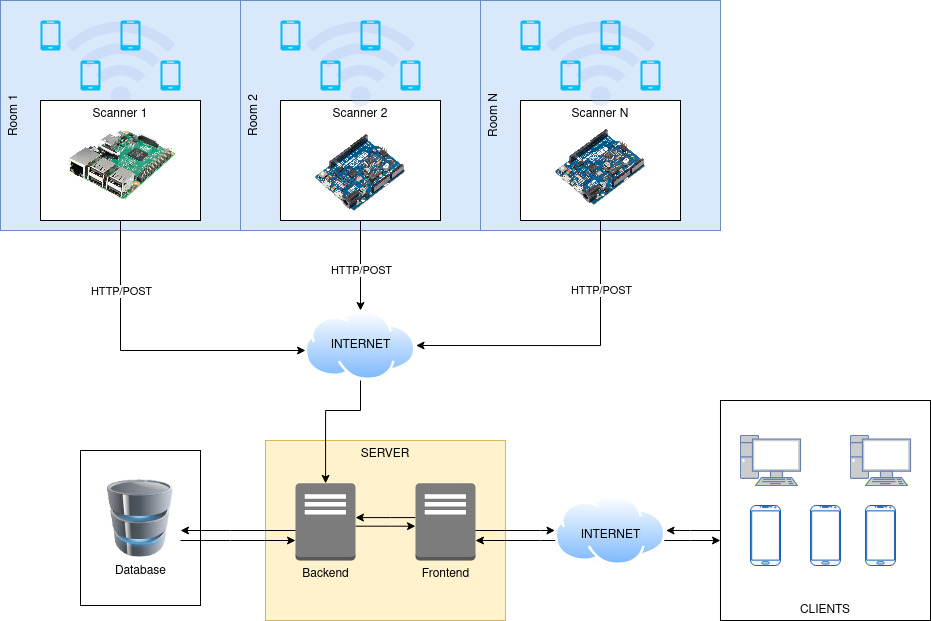
\includegraphics[width=0.7\textwidth]{images/WNMA-ProjectScheme.jpg}
		\caption{System architecture}
	\end{figure}
\end{frame}

\section{Field test}
\begin{frame}{Field test}
	The system has been tested in a real environment: a small local library.
	\begin{itemize}
		\item The scanner (Raspberry Pi) has been placed in a central position
		\item To avoid hosting costs, the server has been deployed on the Raspberry loopback interface
		\item Three days of data collection with few people in the library
	\end{itemize}
\end{frame}

\begin{frame}{Field test}
	\begin{columns}
		% Column 1
		\begin{column}{0.5\textwidth}
			\begin{figure}
				\centering
				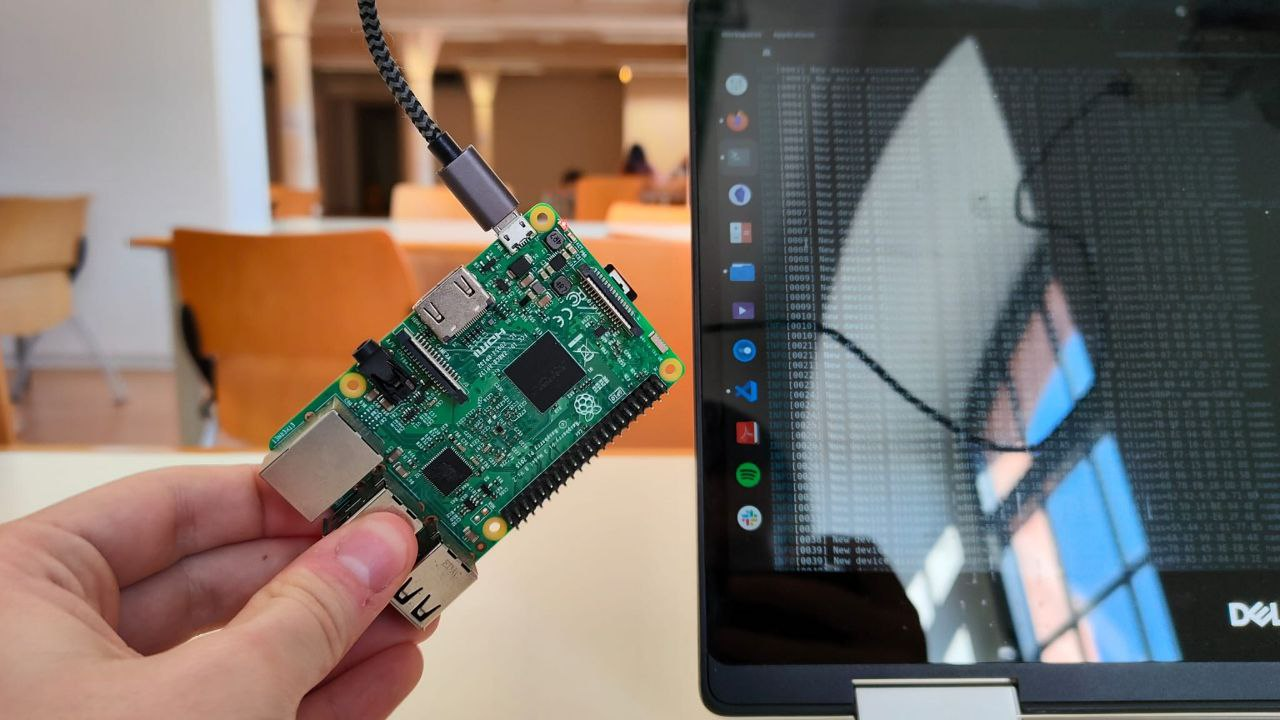
\includegraphics[width=1\textwidth]{images/RpiBiblioPhoto.jpg}
			\end{figure}
		\end{column}
		% Column 2    
		\begin{column}{0.5\textwidth}
			\begin{figure}
				\centering
				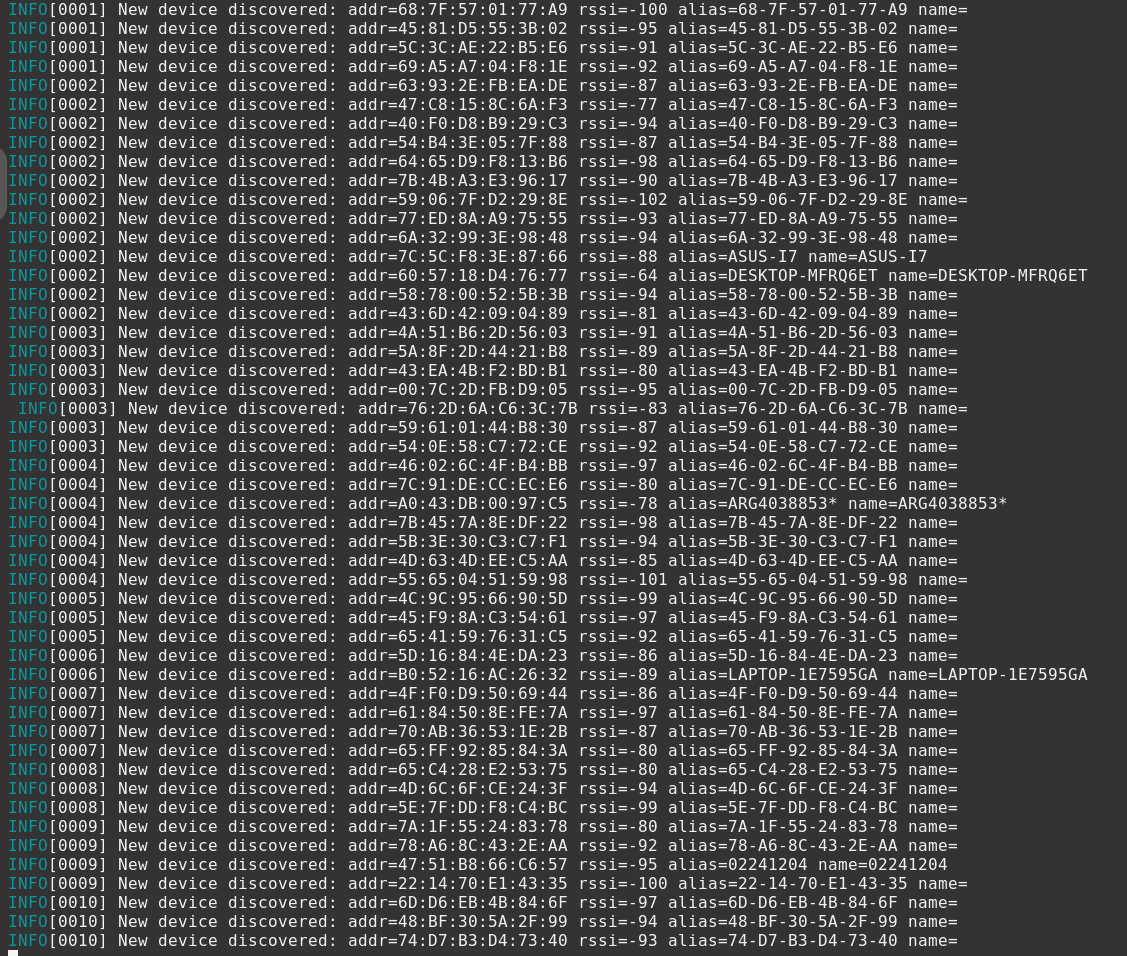
\includegraphics[width=1\textwidth]{images/ScanningScreen.png}
			\end{figure}
		\end{column}
	\end{columns}
\end{frame}


\section{Results}
\begin{frame}{Results}
	\begin{figure}
		\centering
		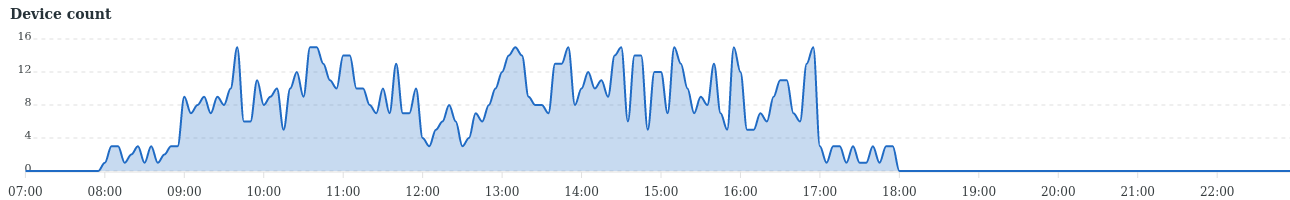
\includegraphics[width=1\textwidth]{images/c1wdhap3.png}
	\end{figure}
	\begin{block}
		{Simple device count}
		\begin{itemize}
			\item High variability in the number of devices detected
			\item occupancy trend is hard to detect
			\item Chart is day-based
		\end{itemize}
	\end{block}
\end{frame}

\begin{frame}{Results}
	\begin{figure}
		\centering
		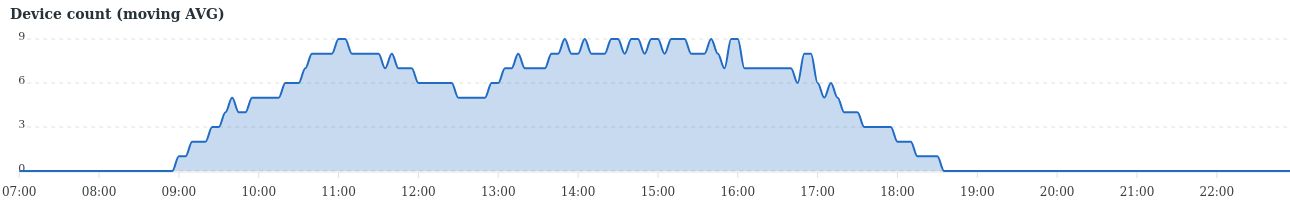
\includegraphics[width=1\textwidth]{images/tp0w3w99f.png}
	\end{figure}
	\begin{block}
		{Moving average device count}
		\begin{itemize}
			\item Moving average with window of 25 minutes
			\item Trend is more visible
		\end{itemize}
		\vspace{1.5em}
		\small{
			\begin{equation}
				{\displaystyle {\begin{aligned}{\textit {SMA}}_{k}&={\frac {p_{n-k+1}+p_{n-k+2}+\cdots +p_{n}}{k}}&={\frac {1}{k}}\sum _{i=n-k+1}^{n}p_{i}\end{aligned}}}
			\end{equation}
		}
	\end{block}
\end{frame}


\begin{frame}[fragile]{Results}
	\begin{figure}
		\centering
		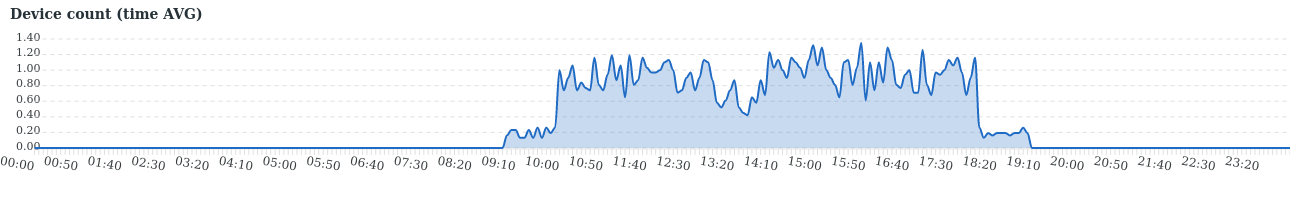
\includegraphics[width=1\textwidth]{images/reyw2zjfg.png}
	\end{figure}
	\begin{block}
		{Average device count per time}
		\begin{lstlisting}[language=SQL]
			SELECT scan.scanTime, COUNT(devices.id) AS numDevices FROM scan
			LEFT JOIN devices ON scan.id = devices.scanID
			WHERE scan.scannerID = ?
			AND scan.scanTime BETWEEN ? AND ?
			GROUP BY scan.scanTime;
		\end{lstlisting}
	\end{block}
\end{frame}

\section{Additional considerations}
\begin{frame}{Additional considerations}
	\textbf{Privacy}
	\begin{itemize}
		\item It may be possible to track user behaviour
		\item Data should be anonymized
		\item MAC randomization by Google and Apple helps
	\end{itemize}
	\vspace{.5em}
	\textbf{Data analysis}: it is possible to further develop the system for advanced analysis of collected data.
	\begin{itemize}
		\item Affluence predictions
		\item Patterns
		\item User behaviour
	\end{itemize}
\end{frame}

\section{Conclusions}
\begin{frame}{Conclusions}
	The prototype has been successfully built as a complete product and seems to work as intended.
	\begin{alertblock}{Problems}
		\begin{itemize}
			\item Test data is insufficient: few days with small amount of people
			\item Not everyone has BT active
			\item People may have multiple BT devices
			\item Results may vary by locations (universities vs post office)
		\end{itemize}
	\end{alertblock}
	\begin{exampleblock}{Conclusions}
		Further test and better data analysis are needed to evaluate the system's effectiveness.
	\end{exampleblock}

\end{frame}

\setbeamercolor{background canvas}{bg=red_unipd}
\begin{frame}{}
	\begin{center}
		\Huge{\textcolor{white}{Thank you for your attention!}}
	\end{center}
\end{frame}

\end{document}
